\section{Vertebrae segmentation}
\subsection{Loss functions}
For multi-class segmentation tasks, different losses are needed. In the case of segmenting specific vertebrae,  the class imbalance is even worse than with the whole spine. 

There is a special type of Dice loss - soft Dice loss, which computes loss for every class separately and then computes the mean. This should work well with small object, as Dice loss does. 

Another loss I was considering was categorical crossentropy loss, which is a generalised version of binary crossentropy for more than 2 classes. I was planning on applying class weights to this loss as well, but unfortunately, Keras does not provide this feature for 2D and 3D volumes. Therefore I focused on the soft Dice loss.

\subsection{Training}
Very similarly to the spine segmentation, I used data split 80/10/10 resulting in 64 training examples, 8 for validation and 8 for testing. It ran on the Google Colab's TPU for 10 hours for 40 epochs. 

The model was trained with soft Dice loss and Adam optimizer, with \textit{learning\_rate}=0.00001. \textit{beta\_1}=0.9, \textit{beta\_2}=0.999 were set by default by the optimizer. The batch size was set to 1 to speed up the training.

In contrast to spine segmentation, the input masks were one-hot-encoded and had dimensions of 96x96x128x26 (26 is the number of classes), where each of the 26 channels represents a segmentation mask for one class. The network outputs a volume of the same dimensions, with probabilities of the pixels to belonging to each of the classes. Probabilities across all classes for one pixel sum to 1. This output is then sent through the argmax function to determine the class (channel) with the highest probability. The result is a segmentation mask of 96x96x128x1, where each element contains the class number. 

\subsection{Results}
The network seemed to be unable to train properly for this task and chosen parameters. The loss would be decreasing for a few epochs, but then got stuck and stayed the same till the rest of the training. I tried overfitting the network only on one image, changing learning rates in the range from 0.001 to 0.000001, with not much success. The losses are in Fig. \ref{fig:loss}. Output of the network was almost all zeros, with a few pixels classified as a vertebrae class. 

\begin{figure}[ht!]
    \centering
    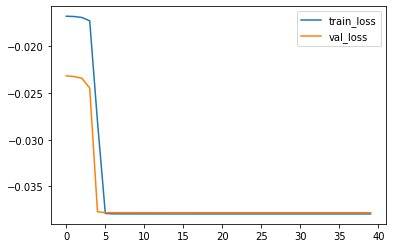
\includegraphics[width=250pt]{images/plot_loss.png}
    \caption[Validation loss]{Validation and train loss across 40 epochs. X axis is number of epochs, Y axis is loss.}
    \label{fig:loss}
\end{figure}

I tried running 2D UNet with the same parameters (only batch size set to 32) to see, if the network is able to learn something, but the results were the same. Loss was decreasing at the beginning, but later stayed the same until the last 40th epoch.

\subsection{Summary}
My network could not be trained for multi-class segmentation problems in either 3D and 2D version. I suspect the problem lays in the choice of the loss function, as it did not work for either of the architectures and the same problem occured for different learning rates. To improve the performance, I could try the before mentioned categorical crossentropy, even though it does not take into account class imbalance. Another approach that could be used is extracting single vertebrae from the images for training.  

